\section{2a. Multicycle Processor}
In this section, we will more go into the detail of the \important{hardware} behind the cpu. Especialy multicycle processor.\\
As seen before, the CPU has more than one part:
\begin{center}
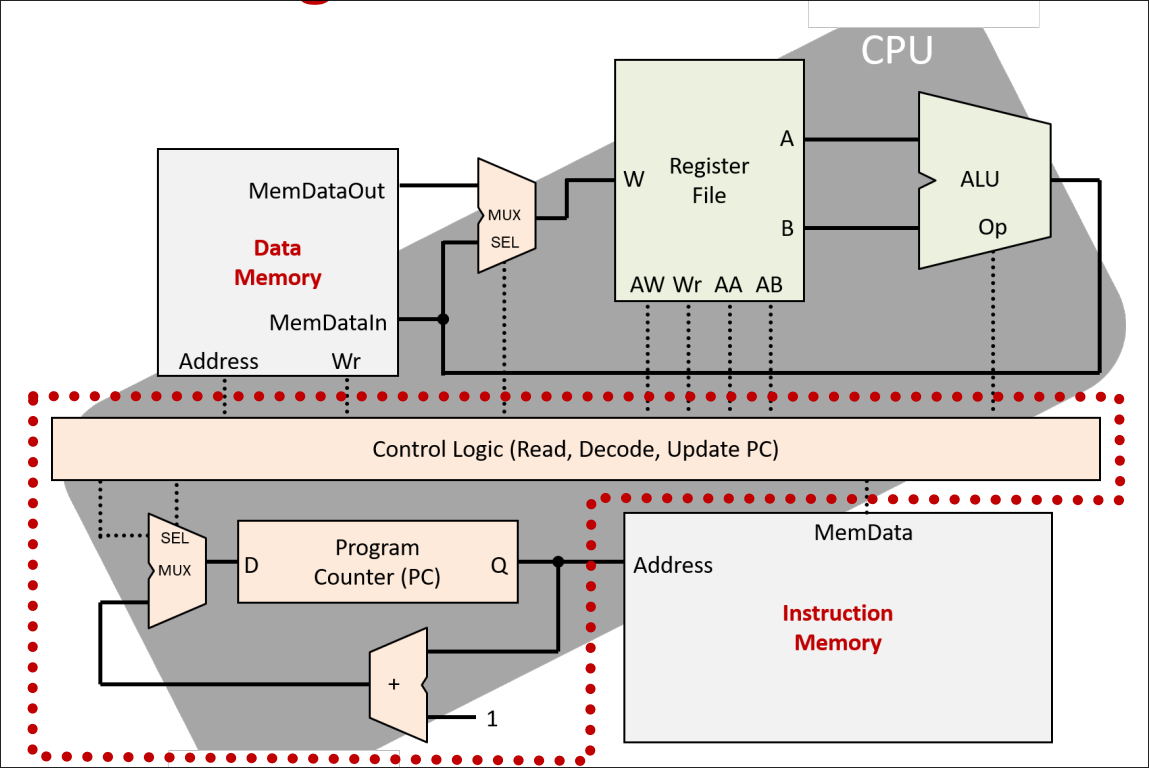
\includegraphics[scale=0.2]{screenshots/2025-10-21_5.png}
\end{center}
However the red part (les pointilles rouges) here is in fact a \important{big finite-state machine}. This means that we can create a state diagram for it.
\begin{parag}{Single cycle processor} For instance the state diagram of a single-cycle processor is very easy: 
\begin{center}
\begin{tikzpicture}[
    state/.style=
	{circle, mininum size=9cm, draw, align=center, ->, >, >=stealth', auto, semithick },
    >=Stealth
]

\node[state]  at (0, 0)(execute) {Execute an\\instruction};
\node[state, right=3cm of execute]at (1, -2) (halt) {Halt};

\draw (execute) edge[loop above] node {PC $\leftarrow$ PC + 4} (exectute);
\draw (halt) edge[loop above] node {not} (halt.west);

\draw[->] (execute) edge[bend left] node {\tt break} (halt);

\end{tikzpicture}
\end{center}
\begin{subparag}{Remark}
    If someone knows how to makes the break here above or below the line I will be curious how.
\end{subparag}
There is only two state which means that every instruction is done at a seperate time (single cycle). This directly implies that the longest \important{combinational path} determines the operating frequncy: \important{critical path}.\\
If we wanted to increase frequency then the critical path would be halved into another cycle.
\end{parag}
\begin{parag}{Two-cycle Processor}
    let us look at the finite state machine of a two cycle processor:
	\begin{center}
	    
	
\begin{tikzpicture}[
    state/.style=
	{circle, mininum size=9cm, draw, align=center, ->, >, >=stealth', auto, semithick },
    >=Stealth
]

% Nodes
\node[state]  at (0, 0)(execute) {Start an\\instruction};
\node[state, right=3cm of execute]at (1, -2) (halt) {Halt};
\node[state, below=2cm of execute] (complete) {Complete the \\ instruction};

% Arrows
% % Loop back arrows
% \draw (execute) edge[bend left] node {not \important{break}} (complete);
% \draw (complete) edge[bend right] node {} (execute);
%
% Break arrow to halt
\draw[->] (execute) edge[bend left] node {\tt break} (halt)
	(execute) edge[bend left] node {not break} (complete)
	 (complete) edge[bend left] (execute);
 \draw[->] (halt) edge[loop below] (halt);
\end{tikzpicture}
\end{center}
The question we must ask now is: Did we gain anything?\\
At the moment not really, before we had 1 instruction \important{per cycle} at frequncy $F$. Now, we have 1 instruction every \important{two cycles} at frequncy $2F$.
\end{parag}
\begin{parag}{Not all paths are born equal}
    That's something sad to say but not all path are born equal, some are slower than other, and this is okay (graine de sarrasins). For instance the \texttt{andi} instruction is much faster than the \texttt{lw} instruction.
\end{parag}
\begin{parag}{Multi cycle Processor}
    




\begin{tikzpicture}[
    stage/.style={
        circle, draw, fill=gray!10,
        minimum size=2cm, align=center
    },
    arrow/.style={
        -{Stealth}, thick
    },
    note/.style={
        rectangle, rounded corners,
        draw=red!70!black, fill=yellow!20,
        very thick, inner sep=10pt, align=left
    }
]

% Nodes (pipeline stages)
\node[stage] (fetch1) {Fetch1};
\node[stage, right=1.8cm of fetch1] (fetch2) {Fetch2};
\node[stage, below right=1.4cm and 1.4cm of fetch2] (decode) {Decode};
\node[stage, below left=1.4cm and 1.4cm of decode] (load1) {Load1};
\node[stage, above left=1.4cm  and 4.6cm of load1] (load2) {Load2};
\node[stage, above left=1.4cm and 1.4cm of load1] (execute) {Execute};

% Arrows between stages
\draw[arrow] (fetch1) edge[bend left] (fetch2);
\draw[arrow] (fetch2) edge[bend left] (decode);
\draw[arrow] (decode) edge[bend left] node[right]{Memory} (load1);
\draw[arrow] (load1) edge[bend left] (load2);
\draw[arrow] (load2)  edge[bend left](fetch1);
\draw[arrow] (decode)  edge[bend left] node[below]{ALU/Branch} (execute);
\draw[arrow] (execute)  edge[bend left](fetch1);

\end{tikzpicture}
\\
The goal here is:
\begin{enumerate}
    \item \important{not} to have \important{too many} stages 
    \item To have paths as \important{balanced} as possible
\end{enumerate}
\end{parag}
\begin{parag}{Mealy or Moore?}
    
\end{parag}
\begin{tikzpicture}[
    block/.style={
        rectangle, rounded corners, draw, thick,
        minimum width=2.6cm, minimum height=1.6cm, align=center
    },
    arrow/.style={-Stealth, thick},
    mybox/.style={
        draw, dashed, rounded corners,
        inner sep=10pt, thick
    },
    labelnode/.style={font=\footnotesize\sffamily}
]

%%% --- MEALY MACHINE (TOP) ---
\node[block, fill=red!10, draw=red!60!black] (next) {Next-State\\Logic\\$f_l[\dots]$};
\node[block, fill=blue!10, draw=blue!70!black, right=2.8cm of next] (state) {State\\Memory};
\node[block, fill=cyan!10, draw=cyan!70!black, right=2.8cm of state] (output) {Output\\Logic\\$g_l[\dots]$};

% Inputs/outputs
\node[left=1.2cm of next] (inputs) {Inputs};
\node[right=1.2cm of output] (outputs) {Outputs};
\node[below=1.1cm of next] (clock1) {Clock};

% Arrows
\draw[arrow] (inputs) -- (next);
\draw[arrow] (next) -- node[above,labelnode]{excitation} (state);
\draw[arrow] (state) -- node[above,labelnode]{current state} (output);
\draw[arrow] (output) -- (outputs);

% Feedback arrows (Mealy)
\draw[arrow, red!70!black, very thick] (inputs.north) to[out=70,in=140,looseness=0.8] (output.west);
\draw[arrow, blue!70!black, very thick] (state.east) to[out=-20,in=270,looseness=0.8] (next.south);
\draw[arrow, blue!70!black, thick] (clock1) -| (state.south west);

% Group box
\node[mybox, fit=(next)(state)(output)] (mealybox) {};
\node[below left=0cm and -0.1cm of mealybox.north west, labelnode] {Mealy Machine};

\pgfdeclarelayer{background}
\pgfsetlayers{background,main}
%%% --- MOORE MACHINE (BOTTOM) ---
\node[block, fill=red!10, draw=red!60!black, below=3.2cm of next] (next2) {Next-State\\Logic\\$f_l[\dots]$};
\node[block, fill=blue!10, draw=blue!70!black, right=2.8cm of next2] (state2) {State\\Memory};
\node[block, fill=cyan!10, draw=cyan!70!black, right=2.8cm of state2] (output2) {Output\\Logic\\$g_l[\dots]$};

% Inputs/outputs
\node[left=1.2cm of next2] (inputs2) {Inputs};
\node[right=1.2cm of output2] (outputs2) {Outputs};
\node[below=1.1cm of next2] (clock2) {Clock};
% Group box
\begin{pgfonlayer}{background}
    
\node[below left=0cm and -0.1cm of moorebox.north west, labelnode] {Moore Machine};
\node[mybox, fill=yellow!15, opacity=0.5, fit=(next2)(state2)(output2)] (moorebox) {};
\end{pgfonlayer}{background}



% Arrows
\draw[arrow] (inputs2) -- (next2);
\draw[arrow] (next2) -- node[above,labelnode]{excitation} (state2);
\draw[arrow] (state2) -- node[above,labelnode]{current state} (output2);
\draw[arrow] (output2) -- (outputs2);

% Feedback arrows (Moore)
\draw[arrow, blue!70!black, thick] (state2.east) to[out=-20,in=270,looseness=0.8] (next2.south);
\draw[arrow, blue!70!black, thick] (clock2) -| (state2.south west);

\end{tikzpicture}
I spent an hour on this so please appreciate.\\
\begin{parag}{$\;$}
    The definition of the mealy fsm is that the output depeneds on the \important{input and state}. On the other hand, the definition of the moore fsm is that the output depends on the \important{state only}. \\
	As a human the moore machine is \textbf{way} easier to develop test, etc. We \textbf{always} want to implement a fsm as a moore machine. And good news: it is always possible (almost)\\
	All we have to do is to retard the current output to the next cycle and put our output as a \textit{state} of the fsm. This way: the next output (which becomes the current) is just a \important{state}.

\end{parag}
\subsection{Building the circuit}

    What we are going to do now is to build the circuit. To do so, we'll do it step by step, adding progressiely what we need.\\
	First, we need an instruction register which store the current instruction (so that it doesn't die after one cycle). We will also need a Controller and the \texttt{pc}.\\

\textbf{I-Type instructions Need \texttt{RF} and \texttt{ALU}}\\
	Type I is the instruction with immediate, this means that there is only one value as input (that's why I put value and not values).
    To be able now to \texttt{add}, \texttt{sub}, etc. We need three things:
	\begin{itemize}
	    \item Value to be computed
	    \item Somewhere to compute
	    \item Value to store the result
	\end{itemize}
	The value to be computed and the value to store the result are in the same place: the \important{register file}. The location where we'll compute the instructions are in the ALU (Arithmetic Logic unit)\\

\textbf{R-Type}\\
	we'll go over instructions with two values as input. To do so, we'll use the same ALU as the one before and we'll just add a multiplexer to choose from the immediate and the register value.\\

\textbf{U-Type instructions write an immediate}\\
    We now need to store immediate instead of the result of the ALU. Therefore, those instructions will need a multiplexer \important{after} the \texttt{ALU} in order to choose to write either the result of the \texttt{ALU} or the immediate.\\

\textbf{Load and Store produces a memory address}\\
    For those we will need to output the address. At  the moment the only \textit{load} that we did is on the program with the \texttt{pc}. However now we will also need to load from the memory data. In order to do this, we will need to choose to load either the pc or the output of the \texttt{ALU} as an address $\implies$ we add a multiplexer.\\

\textbf{Loads write the read data into \texttt{RF}}\\
    So now we can access the memory however after accessing the memory we get a \texttt{rdata} which we still need to manage. To do so we will treat it as it is an output from the \texttt{ALU} by \important{adding} a multiplexer. After this output, we will need a signal to know wether we are choosing from memory or from the ALU \texttt{sel\_mem}.\\

\textbf{Stores send an operant to memory}\\
	Now the instruction we want to implement is the \texttt{sw t0, 16(t1)} instruction. For this instruction, we will choose the \texttt{b} signal as the \texttt{t0} and the \texttt{a} as the address(as we did before). Therefore we need to connect the b into the memory with the new signal \texttt{wdata}. The difference between the store and the load is the \texttt{we} (write enable) signal that serve the memory to know wether we are reading or writing into it.\\

\textbf{Branches need to write an offset to the \texttt{PC}}\\
	 To implement the instruction \texttt{beq t0, t1, 1234}, what we do is to change the \texttt{pc} based on a condition, this condition will be compute in the \texttt{ALU}, the \texttt{alu} will output in his lsb wether or not the \texttt{PC} will be updated.\\
	  If the branch is succesful, we want to replace the current \texttt{PC} by the immediate which leads us to add a path from the controller into the \texttt{PC}, a new branch of the \texttt{imm} signal. The controller has to also informed the \texttt{PC} wether or not we have to enable the writting.\\

	Here we have two clauses:
	\begin{enumerate}
	    \item \texttt{branch\_op} \textrightarrow informs us of if we are in a branch operation 
	    \item \texttt{alu\_res} which is the lsb of the \texttt{ALU} as said before
	\end{enumerate}
	If those two signal are up $\implies$ we enable the write of the \texttt{PC}.
    \begin{framedremark}
    As we can see now, the \texttt{PC} is no longer just a simple register, it contains some logic to compute new values.
    \end{framedremark}
\textbf{jump and link need to store \texttt{PC + 4} in the \texttt{RF}}\\
    To do so, we therefore need another output from the \texttt{PC} which can be stored into the register file based on a signal \texttt{sel\_mem} (whic has to be 0, the inverse of what we have used for before) and the \texttt{sel\_pc} signal.\\
	\begin{center}
	    
	
\scalebox{0.3}{
\begin{circuitikz}
\tikzstyle{every node}=[font=\large]
\draw  (-3.25,30.5) rectangle (3,20.5);
\draw  (-1.25,29.75) rectangle  node {\LARGE Controller} (-1.25,29.75);
\draw  (1.75,29) -- (1.75,29) -- (2.25,29) -- (2.25,29) -- cycle;
\node [font=\Large] at (2,29.75) {sel\_imm};
\node [font=\Large] at (2,28.5) {branch\_op};
\node [font=\Large] at (1.75,28) {rf\_we};
\node [font=\Large] at (1.75,27.5) {sel\_addr};
\node [font=\Large] at (1.75,27) {sel\_b};
\node [font=\Large] at (2,26.5) {sel\_mem};
\node [font=\Large] at (1.75,26) {pc\_en};
\node [font=\Large] at (1.75,25.5) {pc\_sel\_pc\_base};
\node [font=\Large] at (1.5,24.75) {pc\_add\_imm};
\node [font=\Large] at (1.5,24.25) {pc\_sel\_alu};
\node [font=\Large] at (1.75,23.5) {sel\_pc};
\node [font=\Large] at (2,23) {we};
\node [font=\Large] at (2,22.5) {op\_alu};
\node [font=\Large] at (0.75,21) {imm};
\node [font=\Large] at (-1,21) {ir\_en};
\node [font=\Large] at (-2.25,24) {instruction};
\node [font=\Large] at (-2.5,25.5) {rst\_n};
\node [font=\Large] at (-2.5,27.25) {clk};
\draw (3,29.75) to[short] (4.25,29.75);


\draw (7.25,29.75) to[short] (7.5,29.75);
\draw (7.25,29.25) to[short] (7.5,29.25);
\draw (7.5,29.75) node[ieeestd and port, anchor=in 1, scale=0.89](port){} (port.out) to[short] (9.25,29.5);
\draw [ line width=1.7pt](3,29.75) to[short] (7.5,29.75);
\draw [ line width=1.7pt](6.75,29.25) to[short] (7.25,29.25);
\node [font=\Large] at (6,29.25) {alu\_res};
\draw [ line width=1.7pt](3,26) to[short] (10.75,26);
\draw [ line width=1.7pt](10.75,26) to[short] (10.75,29);
\draw [ line width=1.7pt](9.25,29.5) to[short] (10.75,29.5);
\draw (12.5,29.5) to[short] (12.75,29.5);
\draw (12.5,29) to[short] (12.75,29);
\draw (12.75,29.5) node[ieeestd or port, anchor=in 1, scale=0.89](port){} (port.out) to[short] (14.5,29.25);
\draw [ line width=1.7pt](10.75,29) to[short] (12.5,29);
\draw [ line width=1.7pt](10.75,29.5) to[short] (12.75,29.5);
\draw [ line width=1.7pt ] (16.75,31.75) rectangle (23.5,18.5);
\draw [ line width=1.7pt ] (20.5,24.75) rectangle  node {\Huge PC} (20.5,24.75);
\node [font=\Large] at (17.75,31) {clk};
\node [font=\Large] at (17.5,30.25) {rst\_n};
\node [font=\Large] at (17.75,27.5) {};
\node [font=\Large] at (18.25,26.75) {sel\_pb\_base};
\node [font=\Large] at (18.25,26) {add\_imm};
\node [font=\Large] at (18,24.75) {imm};
\node [font=\Large] at (17.75,24.25) {sel\_alu};
\node [font=\Large] at (17.75,23.5) {alu};
\node [font=\Large] at (17.25,29.5) {en};
\draw [ line width=1.7pt](14.5,29.25) to[short] (16.75,29.25);
\draw [ line width=1.7pt](16.75,30.25) to[short] (15.5,30.25);
\draw [ line width=1.7pt](16.75,31.25) to[short] (15.5,31.25);
\draw [ line width=1.7pt](3,25.75) to[short] (15,25.75);
\draw [ line width=1.7pt](16.75,26.75) to[short] (15,26.75);
\draw [ line width=1.7pt](15,26.75) to[short] (15,25.75);
\draw [ line width=1.7pt](16.75,26) to[short] (15.5,26);
\draw [ line width=1.7pt](3,25) to[short] (15.5,25);
\draw [ line width=1.7pt](15.5,26) to[short] (15.5,25);
\draw [ line width=1.7pt](3,24.25) to[short] (16.75,24.25);
\node [font=\Large] at (22.25,19.25) {addr};
\draw [ line width=1.7pt ] (3.25,12.75) rectangle (17.75,4.75);
\draw [ line width=1.7pt ] (-6.25,16) rectangle (-2.25,10.75);
\draw [ line width=1.7pt ] (-4.5,13.75) rectangle  node {\Huge IR} (-4.5,13.75);
\draw [ line width=1.7pt ] (10,8.75) rectangle  node {\Huge Register File} (10,8.75);
\node [font=\Large] at (16.75,11.25) {a};
\node [font=\Large] at (16.75,6.75) {b};
\draw [ line width=1.7pt](21.75,8.25) -- (22.25,8.25);
\draw [ line width=1.7pt](21.75,7.75) -- (22.25,7.75);
\draw [ line width=1.7pt] (22.25,8.75) -- (22.25,7.25) -- (23.25,7.75) -- (23.25, 8.25) -- (22.25,8.75);
\draw [ line width=1.7pt](23.25,8) -- (23.75,8);
\draw [ line width=1.7pt](22.75,9.25) -- (22.75,8.64);
\node [font=\Large] at (22.75,8) {};
\draw [ line width=1.7pt](17.75,6.75) to[short] (21.75,6.75);
\draw [ line width=1.7pt](21.75,7.75) to[short] (21.75,6.75);
\draw [ line width=1.7pt](21.75,8.25) to[short] (19.75,8.25);
\draw [ line width=1.7pt](19.75,8.25) to[short] (19.75,15);
\draw [ line width=1.7pt](19.75,15) to[short] (6.25,15);
\draw [ line width=1.7pt](0.75,20.5) to[short] (0.75,15);
\draw [ line width=1.7pt](6.25,15) to[short] (0.75,15);
\draw [ line width=1.7pt](16.75,25) to[short] (16,25);
\draw [ line width=1.7pt](16,25) to[short] (16,15);
\draw [ line width=1.7pt](16.75,23.5) to[short] (15,23.5);
\node [font=\Large] at (14.25,23.75) {alu\_res};
\node [font=\Large] at (22,9.5) {sel\_b};
\draw [ line width=1.7pt ] (24.75,12.25) rectangle (28.5,6.5);
\draw [ line width=1.7pt ] (26.75,9.75) rectangle  node {\Huge ALU} (26.75,9.75);
\draw [ line width=1.7pt](23.75,8) to[short] (24.75,8);
\draw [ line width=1.7pt](17.75,11.25) to[short] (24.75,11.25);
\draw [ line width=1.7pt](26.75,12.25) to[short] (26.75,14.75);
\node [font=\Large] at (26,14.75) {op\_alu};
\draw [ line width=1.7pt](28.5,9.5) to[short] (32.5,9.5);
\draw [ line width=1.7pt](32.5,9.75) -- (33,9.75);
\draw [ line width=1.7pt](32.5,10.25) -- (33,10.25);
\draw [ line width=1.7pt] (33,9.25) -- (33,10.75) -- (34,10.25) -- (34, 9.75) -- (33,9.25);
\draw [ line width=1.7pt](34,10) -- (34.5,10);
\draw [ line width=1.7pt](33.5,8.75) -- (33.5,9.64);
\node [font=\Large] at (33.5,10) {};
\draw [ line width=1.7pt](32.5,10) to[short] (32.5,9.5);
\draw [ line width=1.7pt](32.5,10.25) to[short] (30.5,10.25);
\node [font=\Large] at (30.5,10.75) {imm};
\node [font=\Large] at (33.25,8.5) {sel\_imm};
\draw [ line width=1.7pt](38.25,9.5) -- (38.75,9.5);
\draw [ line width=1.7pt](38.25,10) -- (38.75,10);
\draw [ line width=1.7pt] (38.75,9) -- (38.75,10.5) -- (39.75,10) -- (39.75, 9.5) -- (38.75,9);
\draw [ line width=1.7pt](39.75,9.75) -- (40.25,9.75);
\draw [ line width=1.7pt](39.25,8.5) -- (39.25,9.39);
\node [font=\Large] at (39.25,9.75) {};
\draw [ line width=1.7pt](34.5,10) to[short] (38.25,10);
\draw [ line width=1.7pt](22.25,18.5) to[short] (22.25,16);
\draw [ line width=1.7pt](22.25,16) to[short] (29,16);
\draw [ line width=1.7pt](29,16) to[short] (29,8.75);
\draw [ line width=1.7pt](29,8.75) to[short] (29,7.5);
\draw [ line width=1.7pt](29.25,7.5) to[short] (31.75,7.5);
\draw [ line width=1.7pt](29.5,7.5) to[short] (29,7.5);
\draw [ line width=1.7pt](32.25,7.25) -- (32.75,7.25);
\draw [ line width=1.7pt](32.25,7.75) -- (32.75,7.75);
\draw [ line width=1.7pt] (32.75,6.75) -- (32.75,8.25) -- (33.75,7.75) -- (33.75, 7.25) -- (32.75,6.75);
\draw [ line width=1.7pt](33.75,7.5) -- (34.25,7.5);
\draw [ line width=1.7pt](33.25,6.25) -- (33.25,7.14);
\node [font=\Large] at (33.25,7.5) {};
\draw [ line width=1.7pt](31.75,7.75) to[short] (32.75,7.75);
\draw [ line width=1.7pt](31.75,7.5) to[short] (31.75,8);
\draw [ line width=1.7pt](34.25,7.5) to[short] (38,7.5);
\draw [ line width=1.7pt](38,7.5) to[short] (38,9.5);
\draw [ line width=1.7pt](38,9.5) to[short] (38.75,9.5);








\node [font=\Large] at (33.25,6) {sel\_mem};



\draw [ line width=1.7pt](40,9.75) to[short] (43.75,9.75);
\draw [ line width=1.7pt](43.75,9.75) to[short] (43.75,4.5);
\draw [ line width=1.7pt](43.75,4.5) to[short] (23.5,4.5);
\draw [ line width=1.7pt](23.5,4.5) to[short] (19.75,4.5);
\draw [ line width=1.7pt](19.75,4.5) to[short] (19.75,2);
\draw [ line width=1.7pt](19.5,2) to[short] (1.75,2);
\draw (39,6.5) to[short] (39,6.75);
\draw (39.5,6.5) to[short] (39.5,6.75);
\draw (39,6.75) node[ieeestd or port, anchor=in 1, scale=0.89, rotate=90](port){} (port.out) to[short] (39.25,8.75);
\node [font=\Large] at (39.75,6.25) {sel\_pc};
\draw [ line width=1.7pt](33.25,6.5) to[short] (39,6.5);
\draw [ line width=1.7pt](29.25,9.5) to[short] (29.25,17.25);
\draw [ line width=1.7pt](30.25,17.25) -- (30.75,17.25);
\draw [ line width=1.7pt](30.25,17.75) -- (30.75,17.75);
\draw [ line width=1.7pt] (30.75,16.75) -- (30.75,18.25) -- (31.75,17.75) -- (31.75, 17.25) -- (30.75,16.75);
\draw [ line width=1.7pt](31.75,17.5) -- (32.25,17.5);
\draw [ line width=1.7pt](31.25,16.25) -- (31.25,17.14);
\node [font=\Large] at (31.25,17.5) {};
\draw [ line width=1.7pt](29.25,17.25) to[short] (30.25,17.25);
\draw [ line width=1.7pt](22.25,17.75) to[short] (30.5,17.75);
\node [font=\Large] at (31.25,16) {sel\_addr};
\draw [ line width=1.7pt](32.25,17.5) to[short] (36.75,17.5);
\node [font=\Large] at (4.25,11.75) {clk};
\node [font=\Large] at (4,10.75) {aa};
\node [font=\Large] at (4,9.75) {ab};
\node [font=\Large] at (3.75,8.75) {aw};
\node [font=\Large] at (4,7.75) {wren};
\node [font=\Large] at (4,6.5) {wrdata};
\draw [ line width=1.7pt](1.75,2) to[short] (1.75,6.5);
\draw [ line width=1.7pt](1.75,6.5) to[short] (3.25,6.5);
\draw [ line width=1.7pt](1,7.75) to[short] (3.25,7.75);
\draw [ line width=1.7pt](0.5,8.75) to[short] (3.25,8.75);
\draw [ line width=1.7pt](-2.25,14.75) to[short] (2,14.75);
\draw [ line width=1.7pt](2,14.75) to[short] (2,10.75);
\draw [ line width=1.7pt](2,10.75) to[short] (3.25,10.75);
\draw [ line width=1.7pt](1,14.75) to[short] (1,9.75);
\draw [ line width=1.7pt](1,9.75) to[short] (3.25,9.75);
\draw [ line width=1.7pt](2.5,11.75) to[short] (3.25,11.75);
\draw [ line width=1.7pt](-0.75,14.75) to[short] (-0.75,10.5);
\draw [ line width=1.7pt](-1.5,14.75) to[short] (-1.5,18.25);
\draw [ line width=1.7pt](-1.5,18.25) to[short] (-4.75,18.25);
\draw [ line width=1.7pt](-4.75,18.25) to[short] (-4.75,23.75);
\draw [ line width=1.7pt](-4.75,23.75) to[short] (-3.25,23.75);
\draw [ line width=1.7pt](-9.25,27.75) to[short] (-3.25,27.75);
\draw [ line width=1.7pt](-9.75,25.5) to[short] (-3.25,25.5);
\draw [ line width=1.7pt](-8,15) to[short] (-6.25,15);
\draw [ line width=1.7pt](-7.75,12) to[short] (-6.25,12);
\end{circuitikz}
}
	\end{center}
	I know it is very ugly but this was \important{loong to do}. (for those intrested I used \url{https://tikzmaker.com}, to do it)

\begin{parag}{Detail complex combinational modules}
	As you can guess each part of those module has more into them, for instance the \texttt{ALU} has 4 sub modules (which we will implement in the first part of the second lab).
    \begin{center}
    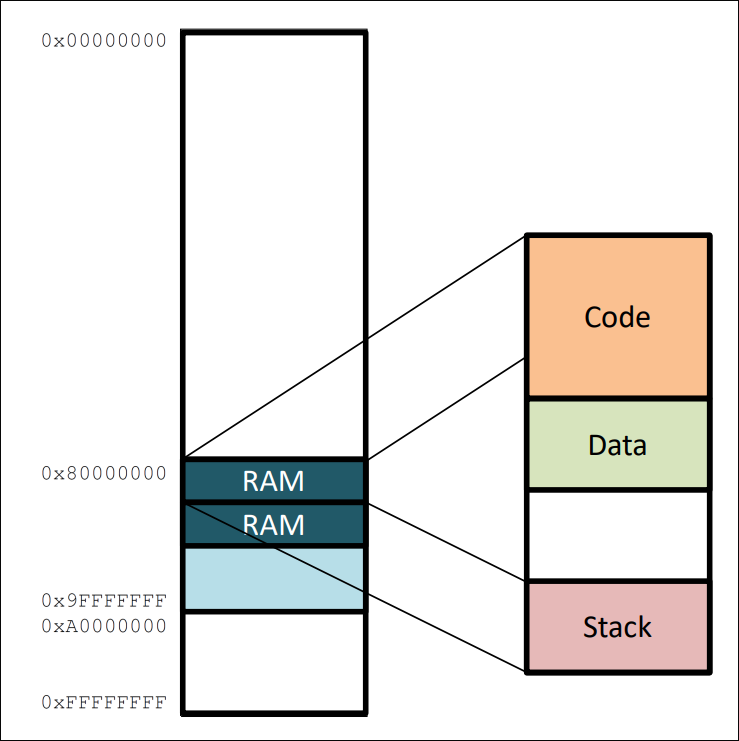
\includegraphics[scale=0.2]{screenshots/2025-10-22_3.png}
    \end{center}
\end{parag}

